\documentclass[aspectratio=169]{beamer}
\usepackage[spanish]{babel}
\usepackage[utf8]{inputenc}
\usepackage{graphicx}
\usepackage{hyperref}
\usepackage{xcolor}

\usetheme{Madrid}
\usecolortheme{dolphin}

\title{Cloud Privado Dinámico}
\subtitle{Proyecto Final de Ciclo}
\author{Moisés Tamaalit Martínez}
\institute{IES Ingeniero de la Cierva}
\date{\today}

\begin{document}

\begin{frame}
\titlepage
\end{frame}

\begin{frame}
\frametitle{Índice}
\tableofcontents
\end{frame}

\section{Introducción}

\begin{frame}
\frametitle{Objetivos del Proyecto}
\begin{itemize}
    \item Desarrollar una plataforma completa de gestión de VPS.
    \item Automatizar el despliegue de servidores virtuales.
    \item Implementar monitorización en tiempo real.
    \item Crear una interfaz de usuario intuitiva.
\end{itemize}
\end{frame}

\section{Arquitectura}

\begin{frame}
\frametitle{Componentes del Sistema}
\begin{columns}
\column{0.5\textwidth}
\begin{itemize}
    \item Frontend (React + TypeScript)
    \item Backend API (Node.js + Express)
    \item API Proxmox (Python + FastAPI)
    \item Base de datos MariaDB
\end{itemize}
\column{0.5\textwidth}
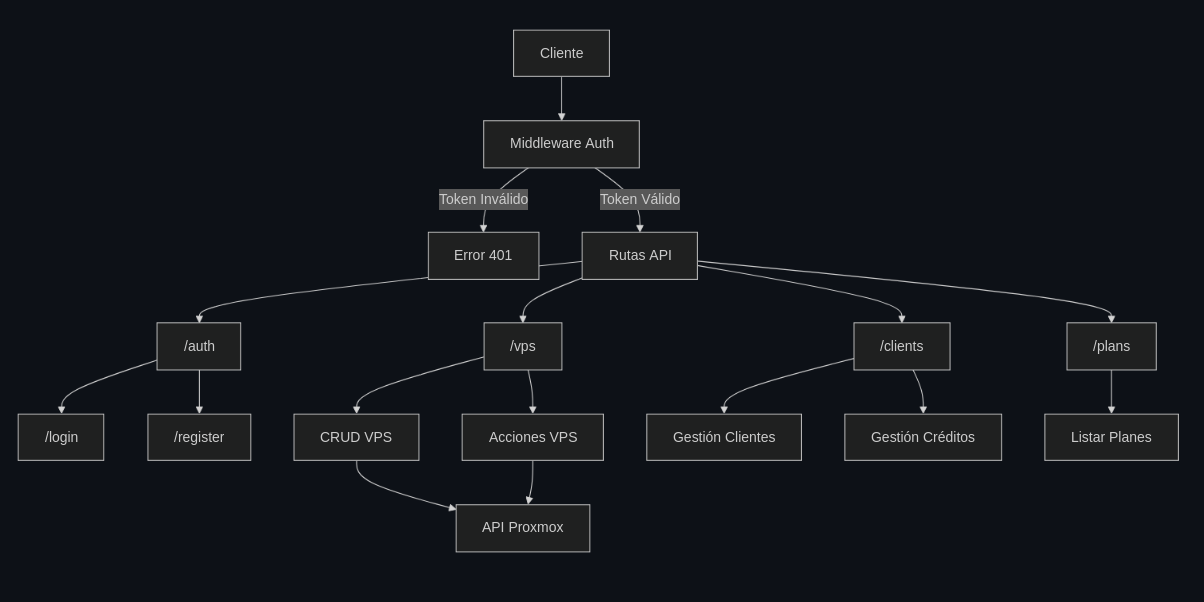
\includegraphics[width=\textwidth]{img/diagrama_backend.png}
\end{columns}
\end{frame}

\begin{frame}
\frametitle{Frontend}
\begin{columns}
\column{0.4\textwidth}
\begin{itemize}
    \item React 19
    \item TypeScript
    \item Tailwind CSS
    \item Shadcn/ui
\end{itemize}
\column{0.6\textwidth}
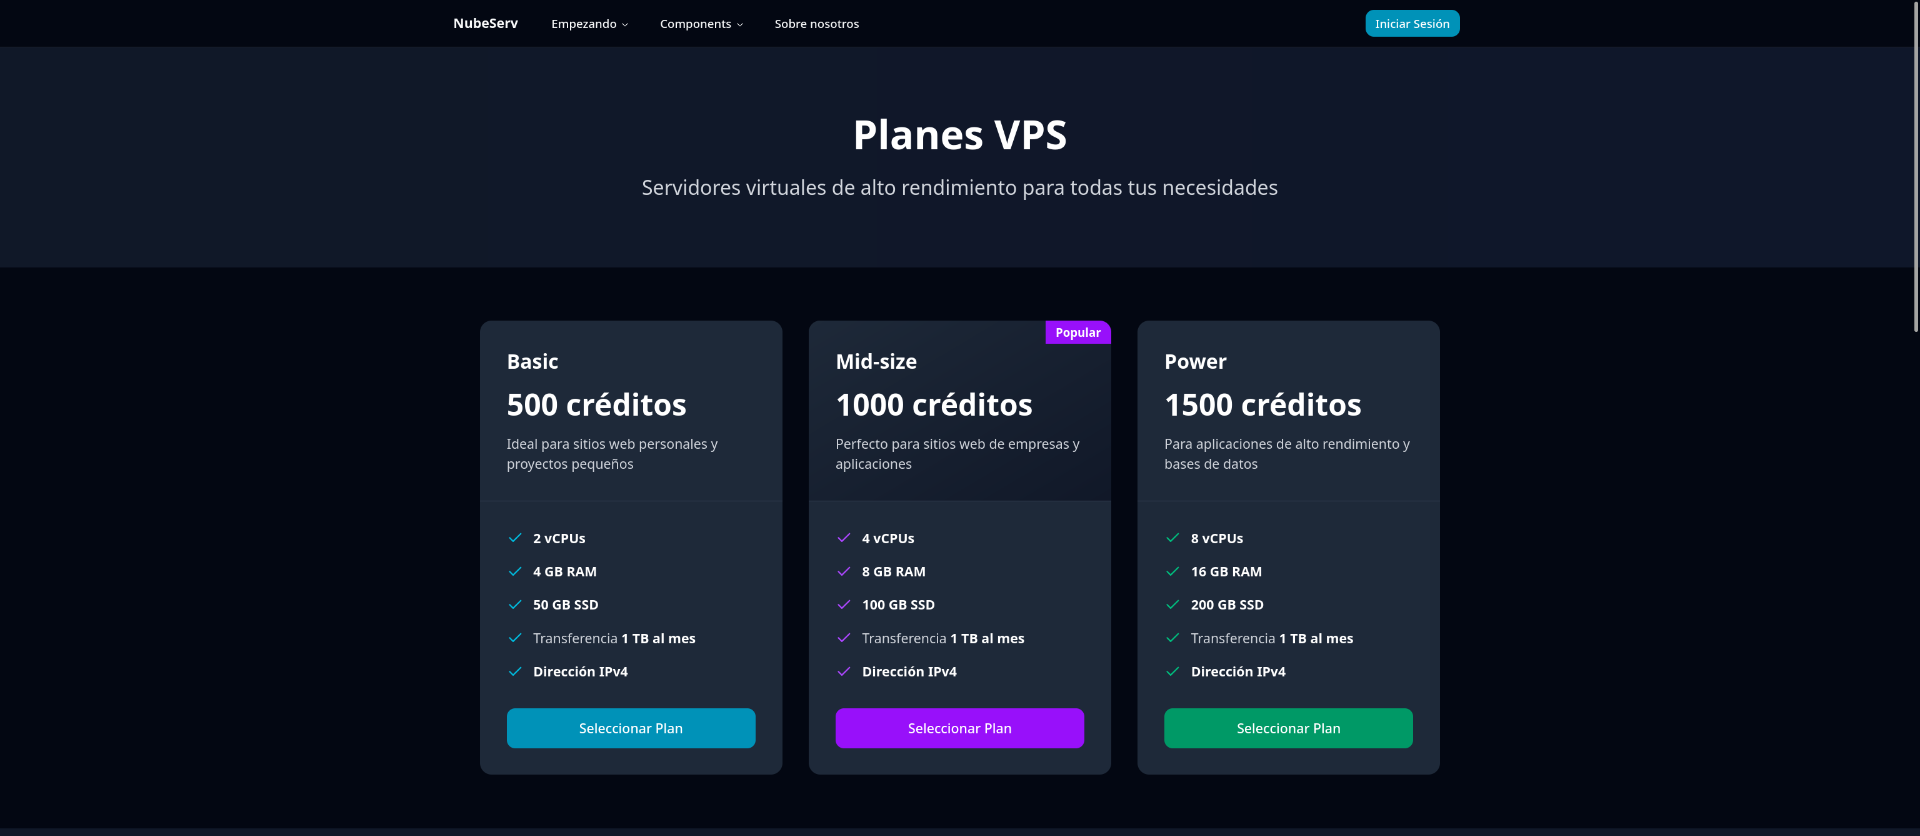
\includegraphics[width=\textwidth]{img/captura_web.png}
\end{columns}
\end{frame}

\begin{frame}
\frametitle{Base de Datos}
\centering
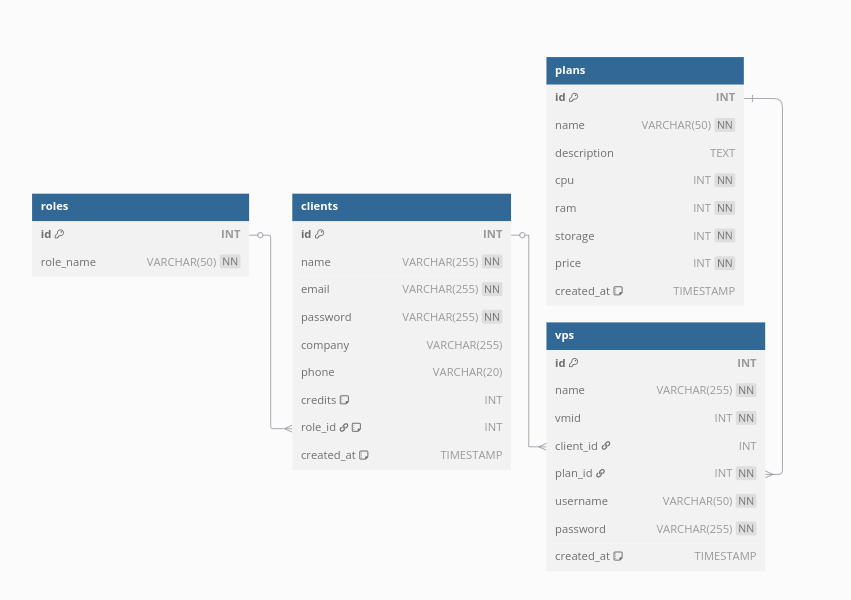
\includegraphics[width=0.9\textwidth]{img/esquema_bd.png}
\end{frame}

\section{Características}

\begin{frame}
\frametitle{Funcionalidades Principales}
\begin{itemize}
    \item Gestión automatizada de VPS
    \item Panel de control intuitivo
    \item Monitorización en tiempo real
    \item Sistema de usuarios y autenticación
\end{itemize}
\end{frame}

\begin{frame}
\frametitle{Seguridad}
\begin{columns}
\column{0.5\textwidth}
\textbf{Autenticación:}
\begin{itemize}
    \item JWT para tokens
    \item Contraseñas con bcrypt
    \item Validación de datos
\end{itemize}
\column{0.5\textwidth}
\textbf{Seguridad VPS:}
\begin{itemize}
    \item Aislamiento de recursos
    \item Redes privadas
    \item Firewall por defecto
\end{itemize}
\end{columns}
\end{frame}

\section{Flujos de Trabajo}

\begin{frame}
\frametitle{Flujo de Cliente}
\centering
% Ajustado a formato vertical manteniendo el aspecto
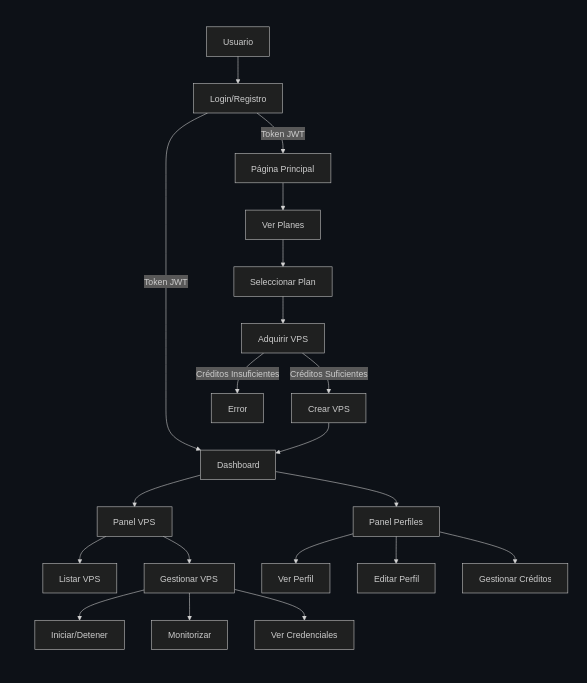
\includegraphics[height=0.8\textheight]{img/diagrama_cliente.png}
\end{frame}

\begin{frame}
\frametitle{Flujo de backend}
\centering
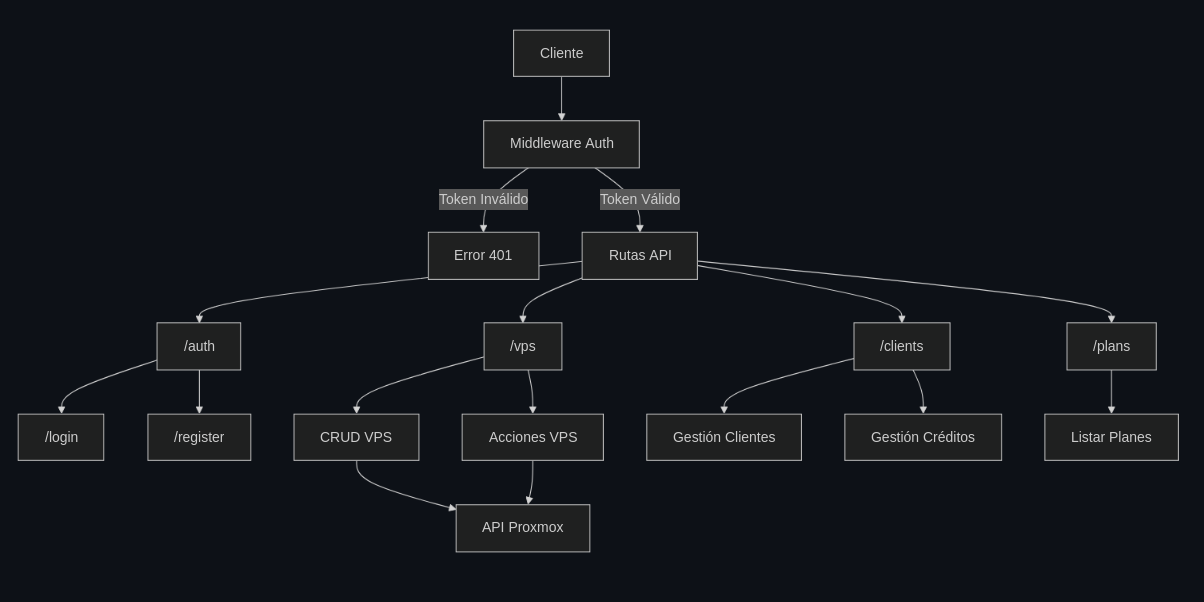
\includegraphics[width=0.8\textwidth]{img/diagrama_backend.png}
\end{frame}

\begin{frame}
\frametitle{Flujo de API Proxmox}
\centering
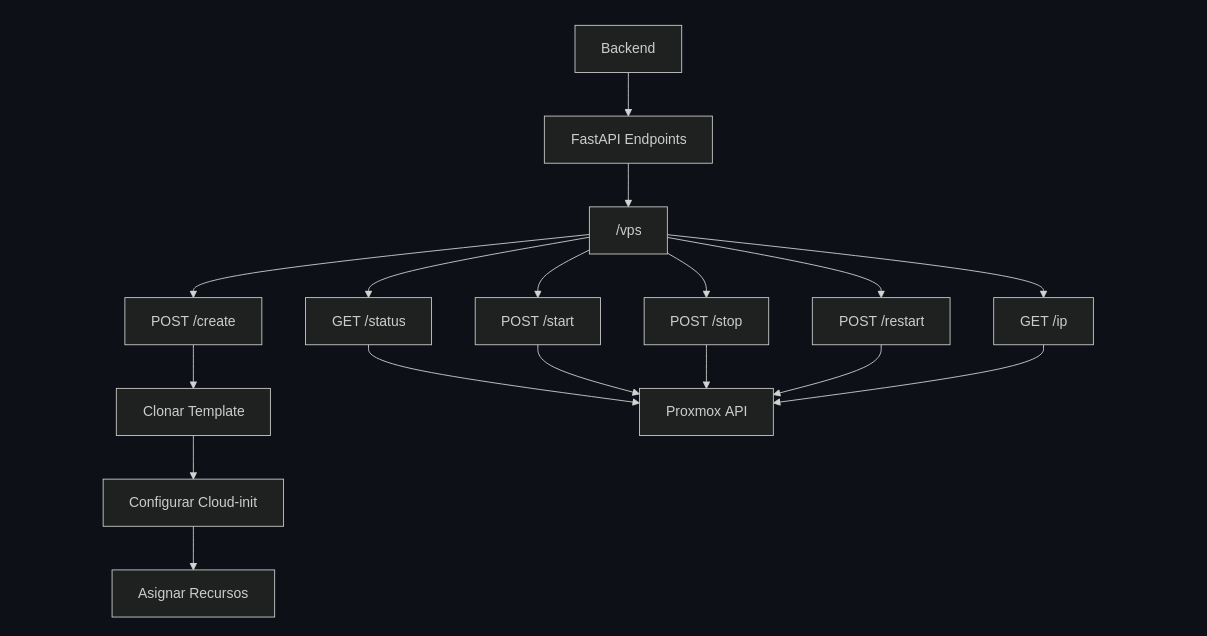
\includegraphics[width=0.8\textwidth]{img/diagrama_proxmox.png}
\end{frame}

\section{Conclusiones}

\begin{frame}
\frametitle{Resultados y Trabajo Futuro}
\begin{columns}
\column{0.5\textwidth}
\textbf{Logros:}
\begin{itemize}
    \item Plataforma funcional
    \item Despliegue automatizado
    \item Interfaz intuitiva
\end{itemize}
\column{0.5\textwidth}
\textbf{Futuro:}
\begin{itemize}
    \item Backups
    \item Métricas avanzadas
    \item API pública
    \item Más hipervisores
\end{itemize}
\end{columns}
\end{frame}

\end{document}
